\chapter{Batched Belief-State Planning}\label{ch:bbmdp}
\chapterquote{Ask not what your \st{country} [GPU] can do for you; ask what you can do for your \st{country} [GPU].}{John F. Kennedy [edited]}

In many real-world decision making problems, an agent must select a single action at each timestep based on limited or uncertain knowledge of its current state.
While the underlying environment may be modeled as a standard Markov decision process (MDP), planning under uncertainty often requires reasoning about multiple possible outcomes or future states.
This motivates the use of \textit{batched planning} methods, in which a set of sampled states are used to evaluate the expected performance of candidate actions.
Such approaches have been widely adopted in belief-space planning \cite{kaelbling1998planning,pineau2003point}, distributionally robust decision making \cite{nilim2005robust,iyengar2005robust}, and batched reinforcement learning algorithms \cite{osband2016deep,lee2021sunrise}, where parallel rollouts are used to compute uncertainty-aware value estimates.
In this chapter, we formalize a batched extension of the MDP used strictly for planning: at each decision step, a single observed state $s$ is duplicated to form a batched representation $\mathbf{s} = \{s, \ldots, s\}$, which is then used to evaluate the expected value of each action under stochastic transitions.
The resulting batched model enables efficient, parallelized rollouts while ensuring that only a single action is selected and executed in the true environment.
The batched planning formulation is motivated by the emphasis on modern GPU architectures for large-scale planning tasks, which can exploit the independence across batches to simulate transitions and compute rewards in parallel with significant speedups \cite{steinkraus2005using}.

\section{Batched Markov Decision Process}\label{sec:batched_mdp}
In this section we formally introduce the batched planning model.
We define the \textit{batched Markov decision process} (\textbf{B}-MDP) as the tuple $\langle \mathcal{S}^m, \mathcal{A}, \mathbf{T}, \widehat{R}, \gamma \rangle$, where the batched state transition function $\mathbf{s}' \sim \mathbf{T}(\cdot \mid \mathbf{s}, a)$ is $\mathbf{T}: \mathcal{S}^m \times \mathcal{A} \to \mathcal{S}^m$, and the set of next states is:
\begin{equation}\label{eq:batched_transition}
    \mathbf{s}' = \big\{s_i'\big\}_{i=1}^m \quad \text{where} \quad s'_i \sim T(\cdot \mid s_i, a) \quad \forall s_i \in \mathbf{s}
\end{equation}
The batched state space $\mathcal{S}^m$ is the multiset of $m$ states:
\begin{equation}
    \mathcal{S}^m = \big\{ \{s_1,s_2,\ldots,s_m\} \mid s_i \in \mathcal{S} \big\}
\end{equation}
with $\mathbf{s} \in \mathcal{S}^m$ denoting a batched state.
The transition function $\mathbf{T}$ can be implemented via a parallelized (e.g., vectorized) form of the standard MDP dynamics.\footnote{In practice, this can be done either through a parallelized simulator, vectorizing the transition function, or a learned neural network surrogate of the transition function for easy GPU vectorization.}
The batched state-based reward function is defined as:
\begin{equation}\label{eq:batched_reward}
    \widehat{R}(\mathbf{s}, \mathbf{a}) = \operatorname*{\mathbb{E}}_{s \in \mathbf{s},\, a \in \mathbf{a}}\big[ R(s,a) \big] = \frac{1}{m}\sum_{i=1}^m R(s_i, a_i)
\end{equation}
where $\mathbf{a} \in \mathcal{A}^m$ denotes batched actions and $m = |\mathbf{s}| = |\mathbf{a}|$ is the batch size.

\subsection{Optimal Batched Value Function}
We show that the batched extension of an MDP preserves the optimality of the value function in the underlying MDP.
The key insight is that, under the batched transition dynamics $\mathbf{T}$, each element $s_i \in \mathbf{s}$ transitions independently according to the underlying MDP transition model, as defined in \cref{eq:batched_transition}.
Similarly, the batched reward function from \cref{eq:batched_reward} is defined as the mean of individual rewards over the batch.
This framework induces a natural decomposition of the batched value function into the average of individual value functions.

Formally, we show that this decomposition leads to the preservation of optimality, namely if $\pi^*$ is an optimal policy for the underlying MDP, then the batched extension $\vec{\pi}^*$ yields a batched value function that is simply the average of optimal state values.
Specifically, the batched value function $\widehat{V}^{\vec{\pi}^*}$ is pointwise optimal over the batch.
We prove this result using the following theorem.

\begin{theorem}[Batched optimal value preservation]\label{thm:batched_value}
Let $\pi: \mathcal{S} \to \mathcal{A}$ be any stationary policy over the underlying MDP, and let $\vec{\pi}: \mathcal{S}^m \to \mathcal{A}^m$ be its batched extension applied independently to each element of $\mathbf{s} \in \mathcal{S}^m$ where $\vec{\pi}(\mathbf{s}) = \{ \pi(s_i) \}_{i=1}^m$. Then the batched value function satisfies:
\begin{equation}
    \widehat{V}^{\vec{\pi}}(\mathbf{s}) = \frac{1}{m} \sum_{i=1}^m V^\pi(s_i)
\end{equation}
and in particular, if $\pi^*$ is optimal for the underlying MDP, then:
\begin{equation}
    \widehat{V}^{\vec{\pi}^*}(\mathbf{s}) = \frac{1}{m} \sum_{i=1}^m V^*(s_i)
\end{equation}
That is, the batched value function preserves optimality in expectation.
\end{theorem}

\begin{proof}
The batched value function under policy $\vec{\pi}$ can be trivially derived as:
\begin{align}
    \widehat{V}^{\vec{\pi}}(\mathbf{s}) 
    &= \mathbb{E}\left[ \sum_{t=0}^\infty \gamma^t \widehat{R}\Big(\mathbf{s}^{(t)}, \vec{\pi}\big(\mathbf{s}^{(t)}\big)\Big) \,\middle|\, \mathbf{s}^{(0)} = \mathbf{s} \right] \\
    &= \mathbb{E}\left[ \sum_{t=0}^\infty \gamma^t \left( \frac{1}{m} \sum_{i=1}^m R\Big(s^{(t)}_i, \pi\big(s^{(t)}_i\big)\Big) \right) \,\middle|\, \big\{s^{(0)}_1, \ldots, s^{(0)}_m\big\} = \mathbf{s} \right] \\
    &= \frac{1}{m} \sum_{i=1}^m \mathbb{E}\left[ \sum_{t=0}^\infty \gamma^t R\Big(s^{(t)}_i, \pi\big(s^{(t)}_i\big)\Big) \,\middle|\, s^{(0)}_i = s_i \right] \\
    &= \frac{1}{m} \sum_{i=1}^m V^\pi(s_i)
\end{align}
If $\pi^*$ is an optimal policy for the underlying MDP, then $V^{\pi^*}(s_i) = V^*(s_i)$ for all $s_i \in \mathcal{S}$. Substituting this into the batched value expression gives:
\begin{equation}\label{eq:batched_value}
    \widehat{V}^{\vec{\pi}^*}(\mathbf{s}) = \frac{1}{m} \sum_{i=1}^m V^*(s_i)
\end{equation}
Thus, the batched value function under the optimal batched policy $\vec{\pi}^*$ is equivalent to the average of the optimal values of the underlying MDP.
Therefore, optimality is preserved under the batched extension in expectation.
\end{proof}

\subsection{Batched Optimal Policy}
This section details how we select optimal independent actions based on the batched value function derived in \cref{eq:batched_value}.
Using the definition of the state-action value (i.e., the $Q$-value) from the underlying MDP, we get:
\begin{equation}
    V^*(s) = \max_{a \in \mathcal{A}} Q^*(s, a)
\end{equation}
Using the results from \cref{thm:batched_value} and applying the definition of the value function from \cref{eq:value_function} (i.e., applying the Bellman operator), we get the following:
\begin{align}
    \widehat{V}^*(\mathbf{s}) 
    &= \frac{1}{m} \sum_{i=1}^m V^*(s_i) \\
    &= \frac{1}{m} \sum_{i=1}^m \max_{a \in \mathcal{A}} Q^*(s_i, a) \\
    &= \frac{1}{m} \sum_{i=1}^m \max_{a \in \mathcal{A}} \left( R(s_i, a) + \gamma \sum_{s'} T(s' \mid s_i, a) V^*(s') \right) \\
    &= \frac{1}{m} \sum_{i=1}^m \max_{a \in \mathcal{A}} \left( R(s_i, a) + \gamma \sum_{s'} T(s' \mid s_i, a) \max_{a' \in \mathcal{A}} Q^*(s', a') \right)
\end{align}
Similarly, we can derive the optimal batched state-action $Q$-value function:
\begin{align}
    \widehat{Q}^*(\mathbf{s}, a) &= \frac{1}{m} \sum_{i=1}^m Q^*(s_i, a) \label{eq:batched_q_value} \\
        &= \frac{1}{m} \sum_{i=1}^m \bigg( R(s_i, a) + \gamma \sum_{s'} T(s' \mid s_i, a) \max_{a' \in \mathcal{A}} Q^*(s', a') \bigg)
\end{align}
We define the optimal batched policy under independent actions as the vector of per-state optimal decisions which captures uncertainty in the per-state dynamics:
\begin{equation}
    \vec{\pi}^*(\mathbf{s}) = \bigg\{ \argmax_{a \in \mathcal{A}} Q^*(s_i, a) \mid s_i \in \mathbf{s} \bigg\}
\end{equation}
This policy defines a batch of locally optimal actions that achieve the maximum value for each individual $s_i$ in the batched planning model.

While $\vec{\pi}^*(\mathbf{s})$ is not a valid execution policy in environments where only one action may be taken, it serves as a useful intermediate representation for analyzing the structure of the batched value function and for planning under independent state samples.
The next section discusses how the batched planning model is used in the true single-state environment.


\section{Batched Planning from a Single State}\label{sec:single_state}

Although the true environment is modeled as a standard MDP $\langle \mathcal{S}, \mathcal{A}, T, R, \gamma \rangle$, in which the agent is only in a single state $s \in \mathcal{S}$ at each timestep and must select a single action $a \in \mathcal{A}$, we formulated the batched planning framework in \cref{sec:batched_mdp} to enable robust and efficient evaluation of potential future outcomes.
This section describes how we use the batched state representation for planning while satisfying the requirement that the agent selects only one action to execute in the true environment.

\subsection{Constructing the Batched Planning Model}
To construct a batched planning representation, we replicate the current state $s$ a total of $m$ times to form a batched state:
\begin{equation}
    \mathbf{s} = \{s, s, \ldots, s\} \in \mathcal{S}^m
\end{equation}
This batched state is used internally for planning purposes, such as simulating forward transitions under stochastic dynamics, evaluating expected returns, or propagating value estimates in parallel.

Transitions and rewards in the batched model follow the independent structure introduced in our formulation of the batched MDP (\cref{sec:batched_mdp}). That is, for a given action $a \in \mathcal{A}$ and duplicated to get $\mathbf{a} = \{a, a, \ldots, a\} \in \mathcal{A}^m$, each element of the batch evolves independently as $s_i' \sim T(\cdot \mid s_i, a_i)$ for each $s_i = s \in \mathbf{s}$ and $a_i = a \in \mathbf{a}$.
The rewards are averaged across the batch as $\widehat{R}(\mathbf{s}, \mathbf{a}) = \frac{1}{m} \sum_{i=1}^m R(s_i, a_i) = R(s, a)$ since all $s_i$ and $a_i$ are identical.

\subsection{Selecting a Single Action}\label{sec:select_single_action}

Although planning is performed over the batched state $\mathbf{s}$ and subsequent batched future states $\mathbf{s}'$, the final policy must ultimately select a single action to execute in the true environment.
We therefore use the batched optimal $Q$-value function to express the single state-action $Q$-value function as:
\begin{equation}
    \widehat{Q}^*(\mathbf{s}, a) = \frac{1}{m} \sum_{i=1}^m Q^*(s_i, a) = Q^*(s, a) \quad \text{for} \quad \mathbf{s} = \{s\}_{i=1}^m
\end{equation}
with $s_i = s$ for all $i$.
This is only true in the degenerate case where all batch elements are identical.
The expansion of $\widehat{Q}^*$ is useful for the general batched planning setting defined in \cref{sec:batched_mdp}, but redundant when $\mathbf{s} = \{s\}_{i=1}^m$.
In the degenerate case, the resulting policy is then given by:
\begin{equation}
    \pi^*(s) = \argmax_{a \in \mathcal{A}} \widehat{Q}^*(\mathbf{s}, a) \quad \text{for} \quad \mathbf{s} = \{s\}_{i=1}^m
\end{equation}
where the recursive definition of $\widehat{Q}^*$ in \cref{eq:batched_q_value} expands each $s \in \mathbf{s}$ based on the transition dynamics.
This policy selects the action that maximizes the expected value across stochastic state transitions from the single known current state.
Importantly, this formulation allows us to use the computational benefits of vectorized or parallelized transitions while maintaining full compatibility with a standard single-agent MDP interface.

\subsection{Interpretation}

The batched formulation can be interpreted as a Monte Carlo approximation of the expected return under stochastic transitions.
Specifically, given a single state $s$ and candidate action $a$, we simulate $m$ stochastic next states $s_i \sim T(\cdot \mid s, a)$ and compute:
\begin{equation}
    \widehat{Q}^*(\mathbf{s}, a) \approx R(s, a) + \gamma \frac{1}{m} \sum_{i=1}^m V^*(s'_i)
\end{equation}
which approximates the Bellman backup:
\begin{equation}
    Q^*(s, a) = R(s, a) + \gamma \mathbb{E}_{s' \sim T(\cdot \mid s, a)} \big[ V^*(s') \big]
\end{equation}
for $s \in \mathbf{s}$.
By evaluating this expectation over $m$ simulated next states, the policy can make informed action choices that account for environmental uncertainty without explicitly modeling a belief state.
This formulation also supports integration with planning algorithms such as Monte Carlo tree search (MCTS) \cite{grill2020monte,cazenave2022batch}, rollout-based policy evaluation \cite{bertsekas2021rollout}, or batched value iteration \cite{ernst2005tree}.
In the next section, we will detail how the batched planning model can be extended to belief-state planning settings.


\begin{figure}[b!]
    \centering
    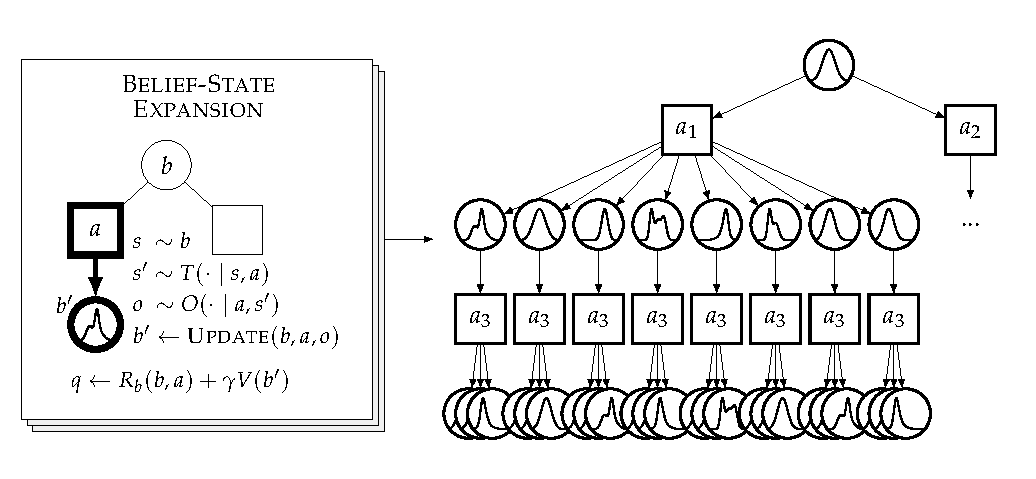
\includegraphics[width=\linewidth]{diagrams/bbmdp/bmdp.pdf}
    \caption{Belief-state MDP for two-step expansion.}
    \label{fig:bmdp_expansion}
\end{figure}


\section{Batched Belief-State Markov Decision Process}
Given a partially observable Markov decision process (POMDP) defined by the tuple $\langle \mathcal{S}, \mathcal{A}, \mathcal{O}, T, R, O, \gamma \rangle$, detailed in \cref{sec:pomdps}, we can convert the POMDP to an equivalent belief-state MDP (see \cref{sec:belief_state_mdps} and \cref{fig:bmdp_expansion}).
Using the batched planning model we derived in \cref{sec:batched_mdp}, we can define the \textit{batched belief-state MDP} (\textbf{BB}-MDP) framework by treating a batch of beliefs $\mathbf{b} = \{b_i\}_{i=1}^m$ as states (shown in \cref{fig:bbmdp_expansion}).
The \textbf{BB}-MDP tuple is defined as $\langle \mathcal{B}^m, \mathcal{A}, \mathbf{T}_b, \widehat{R}_b, \gamma \rangle$, where the batched belief-state transition function $\mathbf{b}' \sim \mathbf{T}_b(\cdot \mid \mathbf{b}, a)$ is $\mathbf{T}_b: \mathcal{B}^m \times \mathcal{A} \to \mathcal{B}^m$, internally computing the following four steps:
\begin{align}
    \mathbf{s}\phantom{'} &= \big\{s_i \big\}_{i=1}^m \quad \text{where} \quad s_i \sim b_i \quad \forall b_i \in \mathbf{b} \label{eq:tbb1} \\ 
    \mathbf{s}' &= \big\{s_i'\big\}_{i=1}^m \quad \text{where} \quad s'_i \sim T(\cdot \mid s_i, a) \quad \forall s_i \in \mathbf{s} \label{eq:tbb2} \\
    \mathbf{o}\phantom{'} &= \big\{o_i\big\}_{i=1}^m \quad \text{where} \quad o_i \sim O(\cdot \mid a, s_i') \quad \forall s_i' \in \mathbf{s}' \label{eq:tbb3} \\
    \mathbf{b}' &= \big\{b'_i\big\}_{i=1}^m \quad \text{where} \quad b_i' \leftarrow \textsc{Update}(b_i, a, o_i) \quad \forall i \in \{1,\ldots,m\} \label{eq:tbb4}
\end{align}
where $b \in \mathcal{B}$ is a belief state belonging to the belief simplex $\mathcal{B}$ over the state space $\mathcal{S}$, and the batched belief state space $\mathcal{B}^m$ is the multiset of $m$ beliefs:
\begin{equation}
    \mathcal{B}^m = \big\{ \{b_1,b_2,\ldots,b_m\} \mid b_i \in \mathcal{B} \big\}
\end{equation}
with $\mathbf{b} \in \mathcal{B}^m$ denoting a batched belief-state.
If the state sampling procedure, the transition function, observation function, and belief update can be done in parallel over batches (e.g., vectorized), this can be simplified to:
\begin{equation}
    \mathbf{s} \sim \mathbf{b} \qquad \mathbf{s}' \sim \mathbf{T}(\cdot \mid \mathbf{s}, a) \qquad \mathbf{o} \sim \mathbf{O}(\cdot \mid a, \mathbf{s}') \qquad \mathbf{b}' = \oldvec{\textsc{Update}}(\mathbf{b}, a, \mathbf{o})    
\end{equation}
for the vectorized transition function $\mathbf{T}: \mathcal{S}^m \times \mathcal{A} \to \mathcal{S}^m$, the vectorized observation function $\mathbf{O}: \mathcal{A} \times \mathcal{S}^m \to \mathcal{O}^m$, and the vectorized belief update function $\oldvec{\textsc{Update}}: \mathcal{B}^m \times \mathcal{A} \times \mathcal{O}^m \to \mathcal{B}^m$.
The batched belief reward function is derived from \cref{eq:batched_reward}:
\begin{align}
    \widehat{R}_b(\mathbf{b}, \mathbf{a}) = \operatorname*{\mathbb{E}}_{b \in \mathbf{b},\, a \in \mathbf{a}} \big[ R_b(b_i, a_i) \big] = \frac{1}{m}\sum_{i=1}^m \left( \int b_i(s) R(s,a_i) \diff s \right)
\end{align}
where $R_b$ is the belief-state reward function defined in \cref{eq:belief_reward}.


\begin{figure}[t]
    \centering
    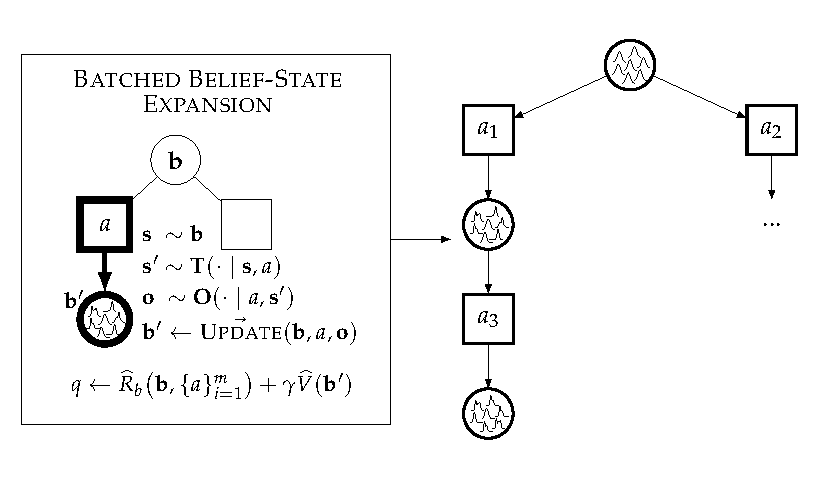
\includegraphics[width=0.75\linewidth]{diagrams/bbmdp/bbmdp.pdf}
    \caption{Batched belief-state MDP for two-step expansion.}
    \label{fig:bbmdp_expansion}
\end{figure}

\subsection{Batched Belief-State Value Function}

To act optimally under partial observability, an agent must evaluate the expected return of a policy $\pi$ given its current belief $b \in \mathcal{B}$.
\textcite{kaelbling1998planning} define the belief-state value function as the expectation of state values weighted by the likelihood under the belief:
\begin{equation}\label{eq:belief_value}
    V^\pi(b) = \int b(s) V^\pi(s) \diff s
\end{equation}
Extending to the batched belief-state model and using the decomposition in \cref{thm:batched_value}, we define the batched belief-state value function as the average value across a batch of beliefs:
\begin{equation}
    \widehat{V}^{\vec{\pi}}(\mathbf{b}) = \frac{1}{m} \sum_{i=1}^m \left( \int b_i(s) V^\pi(s) \diff s\right)
\end{equation}
This value reflects the expected return from executing the policy $\pi$ independently from each belief in the batch, and serves as the basis for value-based planning under state uncertainty.
We can similarly show that when $\pi$ is the optimal policy $\pi^*$, then $\widehat{V}^\pi = \widehat{V}^{\pi^*}$ (following the same argument as \cref{thm:batched_value}).

In the underlying POMDP, the optimal belief-state $Q$-value function is similarly defined as the expected $Q$-value under the belief \cite{kaelbling1998planning}:
\begin{align}
    Q^*(b, a) = \int b(s) Q^*(s,a) \diff s
\end{align}
Extending to the batched planning model, we define the batched belief-state $Q$-value function as the average over the batch of beliefs:
\begin{equation}
    \widehat{Q}^*(\mathbf{b}, a) = \frac{1}{m} \sum_{i=1}^m Q^*(b_i, a) = \frac{1}{m} \sum_{i=1}^m \left( \int b_i(s) Q^*(s, a) \diff s\right)
\end{equation}
This function evaluates the expected return of executing action $a$ across all belief points in the batch $\mathbf{b}$.
The corresponding optimal batched belief-state policy vector is comprised of the actions that maximize the optimal $Q$-value:
\begin{equation}
    \vec{\pi}^*(\mathbf{b}) = \Big\{ \argmax_{a \in \mathcal{A}} Q^*(b_i, a) \mid b_i \in \mathbf{b} \Big\}
\end{equation}

\paragraph{Action selection for a single belief.}
In the outer POMDP loop, when we have a single belief $b$, following \cref{sec:single_state}, we set $\mathbf{b} = \{b\}_{i=1}^m$ as copies of the current belief $b$ to allow the batched planning model to expand in parallel from the current belief.
The action selected at the outer POMDP loop then becomes:
\begin{equation}
    \pi^*(b) = \argmax_{a \in \mathcal{A}} \widehat{Q}^*(\mathbf{b}, a) \quad \text{for} \quad \mathbf{b} = \{b\}_{i=1}^m
\end{equation}
This policy selects a single action that performs well in expectation over the batch of belief states (and their future expansion), enabling robust decision making under state uncertainty.

\subsection{Preliminary Results}
Experimental analysis is provided in the next chapter, yet in \cref{fig:gpu_vs_cpu} we empirically show how sequential scaling compares to batched scaling on an $80$GB NVIDIA A$100$ GPU.
The figure shows an aggregate batch for $n = |\mathcal{A}|$ actions, $m = |\mathbf{b}|$ beliefs per action, and $k = |b|$ states per belief, where we represent each belief $b$ as a collection of state particles $b = \{s_i\}_{i=1}^k$.


\begin{figure}[t!]
    \centering
    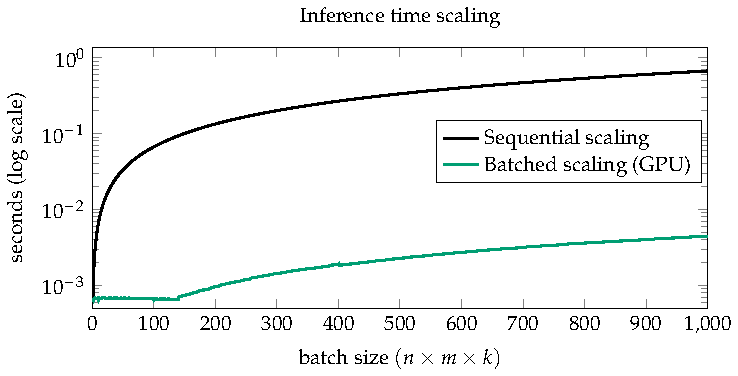
\includegraphics[width=0.855\linewidth]{figures/bbmdp/gpu-vs-cpu}
    \caption{Inference time scaling in \textbf{BB}-MDPs.}
    \label{fig:gpu_vs_cpu}
\end{figure}


\section{Discussion}
In this chapter, we formalized a batched extension to Markov decision processes and belief-state MDPs.
Requirements on a parallelized state transition function and reward function are necessary to adapt standard MDPs to the batched setting.
For POMDPs, in addition to the requirements stated for MDPs, we also require parallelized observation functions and belief updaters.
Future work could focus on batched equivalents for offline planning algorithms such as value iteration (\cref{sec:value_iteration}) and online planning algorithms such as Monte Carlo tree search (\cref{sec:mcts}).
In the next chapter, we will review methods that can be used as parallel belief updaters and introduce a generative surrogate model that approximates the posterior belief through efficient sampling.
